% !TeX program = xelatex
\documentclass{article}
\usepackage{kotex}
\usepackage[a4paper,left=3cm, right=3cm, top=2cm, bottom=2cm]{geometry}
\usepackage{amsmath}
\usepackage{graphicx}
\usepackage{caption}
\usepackage{setspace}
\usepackage{xcolor}
\usepackage{titlesec}
\usepackage{amssymb}
\usepackage{tcolorbox}
\usepackage{wrapfig}
\usepackage{amsthm}
\usepackage{multirow}
\usepackage{array}
\usepackage{tikz}
\usepackage{longtable}
\usepackage{pgfplots}
\pgfplotsset{compat=1.18}

\title{1.1 Introduction to Systems of Linear Equations}
\date{}
\author{}
\setstretch{1.3}

\titleformat{name=\section, numberless}
  {\normalfont\large\bfseries\color{blue}}
  {}
  {0pt}
  {}
\geometry{a4paper, margin=1in}

% Red subheading style (matches the textbook's red section headers)
\newcommand{\redheading}[1]{{\vspace{2mm}\noindent\Large\bfseries\color{red!55!black} #1\par}\vspace{2mm}}

\newtheoremstyle{mystyle}
  {}{}{\itshape}{}{\bfseries}{.}{.5em}{}
\theoremstyle{mystyle}

% Macro for the pseudo-3D "plane" parallelograms used in Figure 1.1.2
\newcommand{\planeA}[3]{
\begin{scope}[shift={(#1,#2)},rotate=#3]
\fill[cyan!12,draw=black,thick] (-1,-0.55) -- (1,-0.55) -- (1.3,0.55) -- (-0.7,0.55) -- cycle;
\end{scope}}

\begin{document}
\section*{Exercise Set 1.1}
\begin{enumerate}
    \item[1.] Determine whether each equation is linear in $x_1, x_2, x_3$.\\
    (a) $x_1+5x_2-\sqrt2\,x_3=1$\quad (b) $x_1+3x_2+x_1x_3=2$\quad (c) $x_1=-7x_2+3x_3$\\
    (d) $x_1^{-2}+x_2+8x_3=5$\quad (e) $x_1^{3/5}-2x_2+x_3=4$\quad (f) $\pi x_1-\sqrt2\,x_2=7^{1/3}$

    \item[3.] Using the notation of Formula (7), write a general linear system with\\
    (a) two equations in two unknowns.\quad (b) three equations in three unknowns.\quad (c) two equations in four unknowns.

    \item[5.] Find a system of linear equations in $x_1,x_2,x_3,\dots$ corresponding to each augmented matrix.\\
    (a) $\begin{bmatrix}2&0&0\\3&-4&0\\0&1&1\end{bmatrix}$\qquad
    (b) $\begin{bmatrix}3&0&-2&5\\7&1&4&-3\\0&-2&1&7\end{bmatrix}$

    \item[7.] Find the augmented matrix for each linear system.\\
    (a) $-2x_1=6,\ 3x_1=8,\ 9x_1=-3$\qquad
    (b) $6x_1-x_2+3x_3=4,\ 5x_2-x_3=1$\\
    (c) $2x_2-3x_4+x_5=0,\ -3x_1-x_2+x_3=-1,\ 6x_1+2x_2-x_3+2x_4-3x_5=6$

    \item[9.] Determine whether each 3-tuple is a solution of
    \[
    2x_1-4x_2-x_3=1,\quad x_1-3x_2+x_3=1,\quad 3x_1-5x_2-3x_3=1
    \]
    (a) $(3,1,1)$\quad (b) $(3,-1,1)$\quad (c) $(13,5,2)$\quad (d) $\left(\tfrac{13}2,\tfrac52,2\right)$\quad (e) $(17,7,5)$

    \item[11.] Solve each system, if possible, and state whether the corresponding lines have zero, one, or infinitely many intersection points; give coordinates or parametric equations accordingly.\\
    (a) $3x-2y=4,\ 6x-4y=9$\qquad (b) $2x-4y=1,\ 4x-8y=2$\qquad (c) $x-2y=0,\ x-4y=8$

    \item[13.] Use parametric equations to describe the solution set of each linear equation.\\
    (a) $7x-5y=3$\quad (b) $3x_1-5x_2+4x_3=7$\quad (c) $-8x_1+2x_2-5x_3+6x_4=1$\quad (d) $3v-8w+2x-y+4z=0$

    \item[15.] Each system below has infinitely many solutions; describe each solution set parametrically.\\
    (a) $2x-3y=1,\ 6x-9y=3$\qquad
    (b) $x_1+3x_2-x_3=-4,\ 3x_1+9x_2-3x_3=-12,\ -x_1-3x_2+x_3=4$

    \item[17.] Find one elementary row operation that creates a 1 in the upper-left corner of the given augmented matrix without introducing fractions in the first row.\\
    (a) $\begin{bmatrix}-3&-1&2&4\\2&-3&3&2\\0&2&-3&1\end{bmatrix}$\qquad
    (b) $\begin{bmatrix}0&-1&-5&0\\2&-9&3&2\\1&4&-3&3\end{bmatrix}$

    \item[19.] Find all values of $k$ for which the given augmented matrix corresponds to a consistent linear system.\\
    (a) $\begin{bmatrix}1&k&-4\\4&8&2\end{bmatrix}$\qquad
    (b) $\begin{bmatrix}1&k&-1\\4&8&-4\end{bmatrix}$

    \item[21.] The curve $y=ax^2+bx+c$ shown passes through $(x_1,y_1),(x_2,y_2),(x_3,y_3)$. Show that $a,b,c$ solve the system with augmented matrix
    \[
    \begin{bmatrix} x_1^2&x_1&1&y_1\\ x_2^2&x_2&1&y_2\\ x_3^2&x_3&1&y_3\end{bmatrix}
    \]
    \begin{figure}[h]
    \centering
    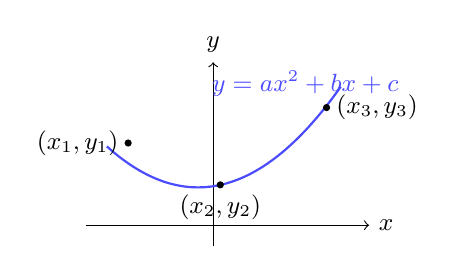
\begin{tikzpicture}[scale=0.9]
    \draw[->] (-1.8,0)--(2.2,0) node[right]{\small$x$};
    \draw[->] (0,-0.3)--(0,2.3) node[above]{\small$y$};
    \draw[blue!70,thick,domain=-1.5:1.8,samples=60] plot(\x,{0.35*\x*\x+0.15*\x+0.55});
    \filldraw[black] (-1.2,1.16) circle (1.2pt) node[left]{\small$(x_1,y_1)$};
    \filldraw[black] (0.1,0.57) circle (1.2pt) node[below]{\small$(x_2,y_2)$};
    \filldraw[black] (1.6,1.66) circle (1.2pt) node[right]{\small$(x_3,y_3)$};
    \node[blue!70] at (1.3,2.0) {\small$y=ax^2+bx+c$};
    \end{tikzpicture}
    \caption*{\textbf{FIGURE Ex-21}}
    \end{figure}

    \item[22.] Explain why none of the three elementary row operations changes the solution set of a linear system.

    \item[23.] Show that if $x_1+kx_2=c$ and $x_1+lx_2=d$ have the same solution set, then $k=l$ and $c=d$.

    \item[25.] A diet requires 7 units of fat, 9 of protein, and 16 of carbohydrates per meal, drawn from three foods (per ounce):\\
    Food 1: 2 fat, 2 protein, 4 carbohydrates.\\
    Food 2: 3 fat, 1 protein, 2 carbohydrates.\\
    Food 3: 1 fat, 3 protein, 5 carbohydrates.\\
    With $x,y,z$ the ounces of foods 1, 2, 3, find (but do not solve) the linear system whose solution gives the required amounts.
\end{enumerate}

\section*{Exercise Set 1.2}
\begin{enumerate}
    \item[1.] Classify each matrix as row echelon form, reduced row echelon form, both, or neither.\\
    (a) $\begin{bmatrix}1&0&0\\0&1&0\\0&0&1\end{bmatrix}$
    (b) $\begin{bmatrix}1&0&0\\0&1&0\\0&0&0\end{bmatrix}$
    (c) $\begin{bmatrix}0&1&0\\0&0&1\\0&0&0\end{bmatrix}$\\[2mm]
    (d) $\begin{bmatrix}1&0&3&1\\0&1&2&4\end{bmatrix}$
    (e) $\begin{bmatrix}1&2&0&3&0\\0&0&1&1&0\\0&0&0&0&1\\0&0&0&0&0\end{bmatrix}$\\[2mm]
    (f) $\begin{bmatrix}0&0\\0&0\\0&0\end{bmatrix}$
    (g) $\begin{bmatrix}1&-7&5&5\\0&1&3&2\end{bmatrix}$

    \item[3.] Each augmented matrix below is a row echelon form reached by row operations. Identify its pivot rows/columns and solve the system.\\
    (a) $\begin{bmatrix}1&-3&4&7\\0&1&2&2\\0&0&1&5\end{bmatrix}$
    (b) $\begin{bmatrix}1&0&8&-5&6\\0&1&4&-9&3\\0&0&1&1&2\end{bmatrix}$\\[2mm]
    (c) $\begin{bmatrix}1&7&-2&0&-8&-3\\0&0&1&1&6&5\\0&0&0&1&3&9\\0&0&0&0&0&0\end{bmatrix}$
    (d) $\begin{bmatrix}1&-3&7&1\\0&1&4&0\\0&0&0&1\end{bmatrix}$

    \item[5.] Solve by Gaussian elimination.\\
    $x_1+x_2+2x_3=8,\quad -x_1-2x_2+3x_3=1,\quad 3x_1-7x_2+4x_3=10$

    \item[7.] Solve by Gaussian elimination.\\
    $x-y+2z-w=-1,\quad 2x+y-2z-2w=-2,\quad -x+2y-4z+w=1,\quad 3x-3w=-3$

    \item[9.] Solve Exercise 5 by Gauss--Jordan elimination.

    \item[11.] Solve Exercise 7 by Gauss--Jordan elimination.

    \item[13.] Determine by inspection (no pencil and paper) whether the homogeneous system has nontrivial solutions.\\
    $2x_1-3x_2+4x_3-x_4=0,\quad 7x_1+x_2-8x_3+9x_4=0,\quad 2x_1+8x_2+x_3-x_4=0$

    \item[15.] Solve by any method.\\
    $2x_1+x_2+3x_3=0,\quad x_1+2x_2=0,\quad x_2+x_3=0$

    \item[17.] Solve by any method.\\
    $3x_1+x_2+x_3+x_4=0,\quad 5x_1-x_2+x_3-x_4=0$

    \item[21.] Solve by any method.\\
    $2I_1-I_2+3I_3+4I_4=9,\quad I_1-2I_3+7I_4=11,\quad 3I_1-3I_2+I_3+5I_4=8,\quad 2I_1+I_2+4I_3+4I_4=10$

    \item[23.] Each augmented matrix below has unspecified entries $*$. Determine whether the system is consistent and, if so, whether the solution is unique -- answer ``inconclusive'' if there isn't enough information.\\
    (a) $\begin{bmatrix}1&*&*&*\\0&1&*&*\\0&0&1&*\end{bmatrix}$
    (b) $\begin{bmatrix}1&*&*&*\\0&1&*&*\\0&0&0&0\end{bmatrix}$
    (c) $\begin{bmatrix}1&*&*&*\\0&1&*&*\\0&0&0&1\end{bmatrix}$
    (d) $\begin{bmatrix}1&*&*&*\\0&0&*&0\\0&0&1&*\end{bmatrix}$

    \item[25.] Determine the values of $a$ for which the system has no solution, exactly one solution, or infinitely many solutions.\\
    $x+2y-3z=4,\quad 3x-y+5z=2,\quad 4x+y+(a^2-14)z=a+2$

    \item[27.] What condition, if any, must $a$, $b$, $c$ satisfy for the system to be consistent?\\
    $x+3y-z=a,\quad x+y+2z=b,\quad 2y-3z=c$

    \item[31.] Find two different row echelon forms of
    \[
    \begin{bmatrix}1&3\\2&7\end{bmatrix}
    \]
    -- showing that row echelon forms need not be unique.

    \item[32.] Reduce
    \[
    \begin{bmatrix}2&1&3\\0&-2&-29\\3&4&5\end{bmatrix}
    \]
    to reduced row echelon form without introducing fractions at any intermediate stage.

    \item[33.] Show that the following nonlinear system has 18 solutions for $0\le\alpha,\beta,\gamma\le2\pi$.
    \[
    \sin\alpha+2\cos\beta+3\tan\gamma=0,\qquad 2\sin\alpha+5\cos\beta+3\tan\gamma=0,\qquad -\sin\alpha-5\cos\beta+5\tan\gamma=0
    \]
    [\emph{Hint:} substitute $x=\sin\alpha$, $y=\cos\beta$, $z=\tan\gamma$.]

    \item[35.] Solve the following nonlinear system for $x,y,z$.
    \[
    x^2+y^2+z^2=6,\qquad x^2-y^2+2z^2=2,\qquad 2x^2+y^2-z^2=3
    \]
    [\emph{Hint:} substitute $X=x^2$, $Y=y^2$, $Z=z^2$.]

    \item[37.] Find $a,b,c,d$ so that the curve shown is the graph of $y=ax^3+bx^2+cx+d$.
    \begin{figure}[h]
    \centering
    \begin{tikzpicture}[scale=0.65]
    \begin{scope}
    \clip (-2.5,-6.1) rectangle (6.7,6.6);
    \draw[->] (-2.4,0)--(6.6,0) node[right]{\small$x$};
    \draw[->] (0,-6)--(0,6.5) node[above]{\small$y$};
    \draw[blue!70,thick,domain=-2.2:6.35,samples=150] plot(\x,{(\x*\x*\x-6*\x*\x+2*\x+10)/6});
    \draw (-0.08,3.333)--(0.08,3.333) node[right]{\scriptsize$20$};
    \draw (-0.08,-3.333)--(0.08,-3.333) node[right]{\scriptsize$-20$};
    \filldraw[black] (0,1.667) circle (1pt) node[above right]{\scriptsize$(0,10)$};
    \filldraw[black] (1,1.167) circle (1pt) node[above right]{\scriptsize$(1,7)$};
    \filldraw[black] (3,-1.833) circle (1pt) node[below]{\scriptsize$(3,-11)$};
    \filldraw[black] (4,-2.333) circle (1pt) node[below right]{\scriptsize$(4,-14)$};
    \node at (-2.1,0.35) {\scriptsize$-2$};
    \node at (6.15,0.35) {\scriptsize$6$};
    \end{scope}
    \end{tikzpicture}
    \caption*{\textbf{FIGURE Ex-37}}
    \end{figure}

    \item[39.] If the linear system
    \[
    a_1x+b_1y+c_1z=0,\qquad a_2x-b_2y+c_2z=0,\qquad a_3x+b_3y-c_3z=0
    \]
    has only the trivial solution, what can be said about the solutions of
    \[
    a_1x+b_1y+c_1z=3,\qquad a_2x-b_2y+c_2z=7,\qquad a_3x+b_3y-c_3z=11\ ?
    \]

    \item[40.] (a) If $A$ has three rows and five columns, what is the maximum possible number of leading 1's in its reduced row echelon form?\\
    (b) If $B$ has three rows and six columns, what is the maximum possible number of parameters in the general solution of the system with augmented matrix $B$?\\
    (c) If $C$ has five rows and three columns, what is the minimum possible number of zero rows in any row echelon form of $C$?

    \item[41.] Describe all possible reduced row echelon forms of\\
    (a) $\begin{bmatrix}a&b&c\\d&e&f\\g&h&i\end{bmatrix}$\qquad
    (b) $\begin{bmatrix}a&b&c&d\\e&f&g&h\\i&j&k&l\\m&n&p&q\end{bmatrix}$
\end{enumerate}

\section*{Exercise Set 1.3}
\begin{enumerate}
    \item[1.] Suppose $A,B,C,D,E$ have sizes $(4\times5),(4\times5),(5\times2),(4\times2),(5\times4)$. Determine whether each expression is defined, and if so, give the size of the result.\\
    (a) $BA$\quad (b) $AB^T$\quad (c) $AC+D$\quad (d) $E(AC)$\quad (e) $A-3E^T$\quad (f) $E(5B+A)$

    \item[3.] Using $A=\begin{bmatrix}3&0\\-1&2\\1&1\end{bmatrix}$, $B=\begin{bmatrix}4&-1\\0&2\end{bmatrix}$, $C=\begin{bmatrix}1&4&2\\3&1&5\end{bmatrix}$, $D=\begin{bmatrix}1&5&2\\-1&0&1\\3&2&4\end{bmatrix}$, $E=\begin{bmatrix}6&1&3\\-1&1&2\\4&1&3\end{bmatrix}$, compute if defined:\\
    (a) $D+E$\ (b) $D-E$\ (c) $5A$\ (d) $-7C$\ (e) $2B-C$\ (f) $4E-2D$\\
    (g) $-3(D+2E)$\ (h) $A-A$\ (i) $\operatorname{tr}(D)$\ (j) $\operatorname{tr}(D-3E)$\ (k) $4\operatorname{tr}(7B)$\ (l) $\operatorname{tr}(A)$

    \item[4.] Using the matrices from Exercise 3, compute if defined:\\
    (a) $2A^T+C$\ (b) $D^T-E^T$\ (c) $(D-E)^T$\ (d) $B^T+5C^T$\ (e) $\tfrac12C^T-\tfrac14A$\ (f) $B-B^T$\\
    (g) $2E^T-3D^T$\ (h) $(2E^T-3D^T)^T$\ (i) $(CD)E$\ (j) $C(BA)$\ (k) $\operatorname{tr}(DE^T)$\ (l) $\operatorname{tr}(BC)$

    \item[7.] Using $A=\begin{bmatrix}3&-2&7\\6&5&4\\0&4&9\end{bmatrix}$, $B=\begin{bmatrix}6&-2&4\\0&1&3\\7&7&5\end{bmatrix}$, use the row or column method to find:\\
    (a) the first row of $AB$\quad (b) the third row of $AB$\quad (c) the second column of $AB$\\
    (d) the first column of $BA$\quad (e) the third row of $AA$\quad (f) the third column of $AA$

    \item[9.] Using $A,B$ from Exercise 7:\\
    (a) Express each column of $AA$ as a linear combination of the columns of $A$.\\
    (b) Express each column of $BB$ as a linear combination of the columns of $B$.

    \item[11.] Find matrices $A,\mathbf{x},\mathbf{b}$ expressing each system as $A\mathbf{x}=\mathbf{b}$, and write out the equation.\\
    (a) $2x_1-3x_2+5x_3=7,\ 9x_1-x_2+x_3=-1,\ x_1+5x_2+4x_3=0$\\
    (b) $4x_1-3x_3+x_4=1,\ 5x_1+x_2-8x_4=3,\ 2x_1-5x_2+9x_3-x_4=0,\ 3x_2-x_3+7x_4=2$

    \item[13.] Express each matrix equation as a system of linear equations.\\
    (a) $\begin{bmatrix}5&6&-7\\-1&-2&3\\0&4&-1\end{bmatrix}\begin{bmatrix}x_1\\x_2\\x_3\end{bmatrix}=\begin{bmatrix}2\\0\\3\end{bmatrix}$\qquad
    (b) $\begin{bmatrix}1&1&1\\2&3&0\\5&-3&-6\end{bmatrix}\begin{bmatrix}x\\y\\z\end{bmatrix}=\begin{bmatrix}2\\2\\-9\end{bmatrix}$

    \item[15.] Find all values of $k$, if any, satisfying
    \[
    \begin{bmatrix}k&1&1\end{bmatrix}\begin{bmatrix}1&1&0\\1&0&2\\0&2&-3\end{bmatrix}\begin{bmatrix}k\\1\\1\end{bmatrix}=0
    \]

    \item[17.] Use the column-row expansion of $AB$ to express the product as a sum of matrix products, for $A=\begin{bmatrix}4&-3\\2&-1\end{bmatrix}$, $B=\begin{bmatrix}0&1&2\\-2&3&1\end{bmatrix}$.

    \item[21.] For the linear system in Example 5 of Section 1.2, express the general solution obtained there as a linear combination of column vectors containing only numerical entries. [\emph{Suggestion:} write the general solution as one column vector, split it into column vectors each containing at most one parameter, then factor out the parameters.]

    \item[23.] Solve for $a,b,c,d$:
    \[
    \begin{bmatrix}a&3\\-1&a+b\end{bmatrix}=\begin{bmatrix}4&d-2c\\d+2c&-2\end{bmatrix}
    \]

    \item[25.] (a) Show that if $A$ has a row of zeros and $B$ is any matrix for which $AB$ is defined, then $AB$ also has a row of zeros.\\
    (b) State and justify a similar result for a column of zeros.

    \item[27.] How many $3\times3$ matrices $A$ satisfy $A\begin{bmatrix}x\\y\\z\end{bmatrix}=\begin{bmatrix}x+y\\x-y\\0\end{bmatrix}$ for \emph{all} $x,y,z$?

    \item[29.] A matrix $B$ is a \textbf{square root} of $A$ if $BB=A$.\\
    (a) Find two square roots of $A=\begin{bmatrix}2&2\\2&2\end{bmatrix}$.\\
    (b) How many different square roots can you find of $A=\begin{bmatrix}5&0\\0&9\end{bmatrix}$?\\
    (c) Do you think every $2\times2$ matrix has at least one square root? Explain.

    \item[30.] Let $0$ denote the $2\times2$ zero matrix.\\
    (a) Is there a $2\times2$ matrix $A\ne0$ with $AA=0$? Justify your answer.\\
    (b) Is there a $2\times2$ matrix $A\ne0$ with $AA=A$? Justify your answer.

    \item[32.] Find a $4\times4$ matrix $A=[a_{ij}]$ satisfying:\\
    (a) $a_{ij}=i+j$\qquad (b) $a_{ij}=i^{j-1}$\qquad
    (c) $a_{ij}=\begin{cases}1 & |i-j|>1\\ -1 & |i-j|\le1\end{cases}$

    \item[33.] Type I, II, III items cost \$1, \$2, \$3 each; the table gives the numbers purchased each month:\\
    \begin{center}
    \begin{tabular}{|l|c|c|c|}
    \hline
     & Type I & Type II & Type III\\
    \hline
    Jan. & 3 & 4 & 3\\
    \hline
    Feb. & 5 & 6 & 0\\
    \hline
    Mar. & 2 & 9 & 4\\
    \hline
    Apr. & 1 & 1 & 7\\
    \hline
    \end{tabular}
    \end{center}
    What does the following product represent?
    \[
    \begin{bmatrix}3&4&3\\5&6&0\\2&9&4\\1&1&7\end{bmatrix}\begin{bmatrix}1\\2\\3\end{bmatrix}
    \]

    \item[35.] \textbf{(Working with Proofs)} Prove: if $A,B$ are $n\times n$, then $\operatorname{tr}(A+B)=\operatorname{tr}(A)+\operatorname{tr}(B)$.
\end{enumerate}

\section*{Exercise Set 1.4}
\begin{enumerate}
    \item[1.] For $A=\begin{bmatrix}3&-1\\2&4\end{bmatrix}$, $B=\begin{bmatrix}0&2\\1&-4\end{bmatrix}$, $C=\begin{bmatrix}4&1\\-3&-2\end{bmatrix}$, $a=4,b=-7$, verify:\\
    (a) the associative law for addition\quad (b) the associative law for multiplication\\
    (c) the left distributive law\quad (d) $(a+b)C=aC+bC$

    \item[3.] Using the matrices from Exercise 1, verify:\\
    (a) $(A^T)^T=A$\qquad (b) $(AB)^T=B^TA^T$

    \item[5.] Use Theorem 1.4.5 to find the inverse of $A=\begin{bmatrix}2&-3\\4&4\end{bmatrix}$.

    \item[10.] Find the inverse of $\begin{bmatrix}\cos\theta&\sin\theta\\-\sin\theta&\cos\theta\end{bmatrix}$.

    \item[13.] For $A=\begin{bmatrix}2&-3\\4&4\end{bmatrix}$, $B=\begin{bmatrix}3&1\\5&2\end{bmatrix}$, $C=\begin{bmatrix}2&0\\0&3\end{bmatrix}$, verify $(ABC)^{-1}=C^{-1}B^{-1}A^{-1}$.

    \item[15.] Given $(7A)^{-1}=\begin{bmatrix}-3&7\\1&-2\end{bmatrix}$, find $A$.

    \item[19.] For $A=\begin{bmatrix}3&1\\2&1\end{bmatrix}$, compute (a) $A^3$\quad (b) $A^{-3}$\quad (c) $A^2-2A+I$.

    \item[21.] For $A=\begin{bmatrix}3&1\\2&1\end{bmatrix}$, compute $p(A)$ for\\
    (a) $p(x)=x-2$\quad (b) $p(x)=2x^2-x+1$\quad (c) $p(x)=x^3-2x+1$

    \item[23.] For $A=\begin{bmatrix}a&b\\c&d\end{bmatrix}$, $B=\begin{bmatrix}0&1\\0&0\end{bmatrix}$, find all $a,b,c,d$ for which $A,B$ commute.

    \item[25.] Use the method of Example 8 to find the unique solution of\\
    $3x_1-2x_2=-1,\quad 4x_1+5x_2=3$

    \item[30.] Verify $p(A)=p_1(A)p_2(A)$ for $p(x)=x^2-9=(x+3)(x-3)$ and an arbitrary square matrix $A$.

    \item[31.] (a) Give an example of $2\times2$ matrices with $(A+B)(A-B)\ne A^2-B^2$.\\
    (b) State a valid formula for $(A+B)(A-B)$.\\
    (c) What condition on $A,B$ allows $(A+B)(A-B)=A^2-B^2$?

    \item[32.] The equation $a^2=1$ has exactly two real solutions. Find at least eight solutions of $A^2=I_3$. [\emph{Hint:} look for solutions with all off-diagonal entries zero.]

    \item[33.] (a) Show that if $A^2+2A+I=0$, then $A$ is invertible; find $A^{-1}$.\\
    (b) Show that if $p(x)$ has nonzero constant term and $p(A)=0$, then $A$ is invertible.

    \item[34.] Is it possible for $A^3$ to equal the identity matrix without $A$ being invertible? Explain.

    \item[35.] Can a matrix with a zero row or column have an inverse? Explain.

    \item[36.] Can a matrix with two identical rows or columns have an inverse? Explain.

    \item[37.] Determine whether $A=\begin{bmatrix}1&0&1\\1&1&0\\0&1&1\end{bmatrix}$ is invertible, and if so find $A^{-1}$. [\emph{Hint:} solve $AX=I$ for $X$ by equating corresponding entries.]

    \item[39.] Simplify, assuming $A,B,C,D$ invertible: $(AB)^{-1}(AC^{-1})(D^{-1}C^{-1})^{-1}D^{-1}$.

    \item[41.] Show that if $R$ is $1\times n$ and $C$ is $n\times1$, then $RC=\operatorname{tr}(CR)$.

    \item[43.] (a) Show that if $A$ is invertible and $AB=AC$, then $B=C$.\\
    (b) Explain why part (a) and Example 3 do not contradict each other.

    \item[45.] (a) Show that if $A,B,A+B$ are invertible matrices of the same size, then $A(A^{-1}+B^{-1})B(A+B)^{-1}=I$.\\
    (b) What does part (a) tell you about the matrix $A^{-1}+B^{-1}$?

    \item[46.] A square matrix $A$ is \textbf{idempotent} if $A^2=A$.\\
    (a) Show that if $A$ is idempotent, so is $I-A$.\\
    (b) Show that if $A$ is idempotent, then $2A-I$ is invertible and is its own inverse.

    \item[47.] Show that if $A^k=0$ for some positive integer $k$, then $I-A$ is invertible and $(I-A)^{-1}=I+A+A^2+\cdots+A^{k-1}$.

    \item[48.] Show that $A=\begin{bmatrix}a&b\\c&d\end{bmatrix}$ satisfies $A^2-(a+d)A+(ad-bc)I=0$.

    \item[51.] \textbf{(Working with Proofs)} Prove Theorem 1.4.1(a).
\end{enumerate}

\section*{Exercise Set 1.5}
\begin{enumerate}
    \item[1.] Determine whether the matrix is elementary.\\
    (a) $\begin{bmatrix}1&0\\-5&1\end{bmatrix}$\quad (b) $\begin{bmatrix}-5&1\\1&0\end{bmatrix}$\quad (c) $\begin{bmatrix}1&1&0\\0&0&1\\0&0&0\end{bmatrix}$\quad (d) $\begin{bmatrix}2&0&0&2\\0&1&0&0\\0&0&1&0\\0&0&0&1\end{bmatrix}$

    \item[3.] Find a row operation and its elementary matrix that restores the given elementary matrix to $I$.\\
    (a) $\begin{bmatrix}1&-3\\0&1\end{bmatrix}$\quad (b) $\begin{bmatrix}-7&0&0\\0&1&0\\0&0&1\end{bmatrix}$\quad (c) $\begin{bmatrix}1&0&0\\0&1&0\\-5&0&1\end{bmatrix}$\quad (d) $\begin{bmatrix}0&0&1&0\\0&1&0&0\\1&0&0&0\\0&0&0&1\end{bmatrix}$

    \item[5.] Identify the row operation corresponding to $E$ and verify that $EA$ results from applying it to $A$.\\
    (a) $E=\begin{bmatrix}0&1\\1&0\end{bmatrix}$, $A=\begin{bmatrix}-1&-2&5&-1\\3&-6&-6&-6\end{bmatrix}$\\
    (b) $E=\begin{bmatrix}1&0&0\\0&1&0\\0&-3&1\end{bmatrix}$, $A=\begin{bmatrix}2&-1&0&-4&-4\\1&-3&-1&5&3\\2&0&1&3&-1\end{bmatrix}$\\
    (c) $E=\begin{bmatrix}1&0&4\\0&1&0\\0&0&1\end{bmatrix}$, $A=\begin{bmatrix}1&4\\2&5\\3&6\end{bmatrix}$

    \item[7.] Using $A=\begin{bmatrix}3&4&1\\2&-7&-1\\8&1&5\end{bmatrix}$, $B=\begin{bmatrix}8&1&5\\2&-7&-1\\3&4&1\end{bmatrix}$, $C=\begin{bmatrix}3&4&1\\2&-7&-1\\2&-7&3\end{bmatrix}$, find an elementary matrix $E$ satisfying:\\
    (a) $EA=B$\quad (b) $EB=A$\quad (c) $EA=C$\quad (d) $EC=A$

    \item[9.] First use Theorem 1.4.5, then the inversion algorithm, to find $A^{-1}$ if it exists.\\
    (a) $A=\begin{bmatrix}1&4\\2&7\end{bmatrix}$\qquad (b) $A=\begin{bmatrix}2&-4\\-4&8\end{bmatrix}$

    \item[11.] Use the inversion algorithm to find the inverse, if it exists.\\
    (a) $\begin{bmatrix}1&2&3\\2&5&3\\1&0&8\end{bmatrix}$\qquad (b) $\begin{bmatrix}-1&3&-4\\2&4&1\\-4&2&-9\end{bmatrix}$

    \item[13.] Use the inversion algorithm to find the inverse, if it exists, of $\begin{bmatrix}1&0&1\\0&1&1\\1&1&0\end{bmatrix}$.

    \item[19.] Find the inverse of each $4\times4$ matrix, where $k_1,k_2,k_3,k_4,k$ are all nonzero.\\
    (a) $\begin{bmatrix}k_1&0&0&0\\0&k_2&0&0\\0&0&k_3&0\\0&0&0&k_4\end{bmatrix}$\qquad
    (b) $\begin{bmatrix}k&1&0&0\\0&1&0&0\\0&0&k&1\\0&0&0&1\end{bmatrix}$

    \item[21.] Find all values of $c$, if any, for which the matrix is invertible.
    \[
    \begin{bmatrix}c&c&c\\1&c&c\\1&1&c\end{bmatrix}
    \]

    \item[23.] Express the matrix and its inverse as products of elementary matrices.
    \[
    \begin{bmatrix}-3&1\\2&2\end{bmatrix}
    \]

    \item[27.] Show that $A=\begin{bmatrix}1&2&3\\1&4&1\\2&1&9\end{bmatrix}$ and $B=\begin{bmatrix}1&0&5\\0&2&-2\\1&1&4\end{bmatrix}$ are row equivalent by finding a sequence of elementary row operations that produces $B$ from $A$, and use it to find a matrix $C$ with $CA=B$.

    \item[29.] Show that if $A=\begin{bmatrix}1&0&0\\0&1&0\\a&b&c\end{bmatrix}$ is an elementary matrix, then at least one entry in the third row must be zero.

    \item[30.] Show that
    \[
    A=\begin{bmatrix}0&a&0&0&0\\b&0&c&0&0\\0&d&0&e&0\\0&0&f&0&g\\0&0&0&h&0\end{bmatrix}
    \]
    is not invertible for any values of the entries.

    \item[31.] \textbf{(Working with Proofs)} Prove that if $A,B$ are $m\times n$ matrices, then $A,B$ are row equivalent if and only if they have the same reduced row echelon form.

    \item[32.] \textbf{(Working with Proofs)} Prove that if $A$ is invertible and $B$ is row equivalent to $A$, then $B$ is also invertible.

    \item[33.] \textbf{(Working with Proofs)} Prove that if $B$ is obtained from $A$ by a sequence of elementary row operations, then a second sequence of elementary row operations, applied to $B$, recovers $A$.
\end{enumerate}

\section*{Exercise Set 1.6}
\begin{enumerate}
    \item[1.] Solve by inverting the coefficient matrix and using Theorem 1.6.2.\\
    $x_1+x_2=2,\quad 5x_1+6x_2=9$

    \item[3.] $x_1+3x_2+x_3=4,\quad 2x_1+2x_2+x_3=-1,\quad 2x_1+3x_2+x_3=3$

    \item[6.] $-x-2y-3z=0,\quad w+x+4y+4z=7,\quad w+3x+7y+9z=4,\quad -w-2x-4y-6z=6$

    \item[7.] Solve for $x_1,x_2$ in terms of $b_1,b_2$: $3x_1+5x_2=b_1,\quad x_1+2x_2=b_2$

    \item[9.] Solve the linear systems together by reducing an appropriate augmented matrix to reduced row echelon form.\\
    $x_1-5x_2=b_1,\quad 3x_1+2x_2=b_2$\\
    (i) $b_1=1,b_2=4$\qquad (ii) $b_1=-2,b_2=5$

    \item[13.] Determine conditions on the $b_i$'s, if any, for the system to be consistent.\\
    $x_1+3x_2=b_1,\quad -2x_1+x_2=b_2$

    \item[15.] $x_1-2x_2+5x_3=b_1,\quad 4x_1-5x_2+8x_3=b_2,\quad -3x_1+3x_2-3x_3=b_3$

    \item[18.] For $A=\begin{bmatrix}2&1&2\\2&2&-2\\3&1&1\end{bmatrix}$, $\mathbf{x}=\begin{bmatrix}x_1\\x_2\\x_3\end{bmatrix}$:\\
    (a) Show that $A\mathbf{x}=\mathbf{x}$ can be rewritten as $(A-I)\mathbf{x}=\mathbf{0}$, and use this to solve $A\mathbf{x}=\mathbf{x}$.\\
    (b) Solve $A\mathbf{x}=4\mathbf{x}$.

    \item[19.] Solve the matrix equation for $X$.
    \[
    \begin{bmatrix}1&-1&1\\2&3&0\\0&2&-1\end{bmatrix}X=\begin{bmatrix}2&-1&5&7&8\\4&0&-3&0&1\\3&5&-7&2&1\end{bmatrix}
    \]

    \item[21.] \textbf{(Working with Proofs)} Let $A\mathbf{x}=\mathbf{0}$ be a homogeneous system of $n$ equations in $n$ unknowns with only the trivial solution. Prove that for any positive integer $k$, $A^k\mathbf{x}=\mathbf{0}$ also has only the trivial solution.

    \item[23.] \textbf{(Working with Proofs)} Let $A\mathbf{x}=\mathbf{b}$ be any consistent system, and let $\mathbf{x}_1$ be a fixed solution. Prove that every solution can be written $\mathbf{x}=\mathbf{x}_1+\mathbf{x}_0$ where $\mathbf{x}_0$ solves $A\mathbf{x}=\mathbf{0}$, and that every matrix of this form is a solution.

    \item[24.] \textbf{(Working with Proofs)} Use part (a) of Theorem 1.6.3 to prove part (b).
\end{enumerate}

\section*{Exercise Set 1.7}
\begin{enumerate}
    \item[1.] Classify each matrix as upper triangular, lower triangular, diagonal (note: a diagonal matrix is both), or none of these.\\[2pt]
    (a) $\begin{bmatrix}2&1\\0&3\end{bmatrix}$\quad
    (b) $\begin{bmatrix}0&0\\4&0\end{bmatrix}$\quad
    (c) $\begin{bmatrix}-1&0&0\\0&2&0\\0&0&\frac{1}{5}\end{bmatrix}$\quad
    (d) $\begin{bmatrix}3&-2&7\\0&0&3\\0&0&8\end{bmatrix}$

    \item[3.] Find the product by inspection (using the diagonal multiplication rule).
    \[
    \begin{bmatrix}3&0&0\\0&-1&0\\0&0&2\end{bmatrix}\begin{bmatrix}2&1\\-4&1\\2&5\end{bmatrix}
    \]

    \item[7.] Find $A^2$, $A^{-2}$, and $A^{-k}$ (where $k$ is any integer) by inspection.
    \[
    A=\begin{bmatrix}1&0\\0&-2\end{bmatrix}
    \]

    \item[8.] Find $A^2$, $A^{-2}$, and $A^{-k}$ by inspection.
    \[
    A=\begin{bmatrix}-6&0&0\\0&3&0\\0&0&5\end{bmatrix}
    \]

    \item[11.] Compute the product by inspection.
    \[
    \begin{bmatrix}1&0&0\\0&0&0\\0&0&3\end{bmatrix}
    \begin{bmatrix}2&0&0\\0&5&0\\0&0&0\end{bmatrix}
    \begin{bmatrix}0&0&0\\0&2&0\\0&0&1\end{bmatrix}
    \]

    \item[13.] Compute the indicated power by inspection.
    \[
    \begin{bmatrix}1&0\\0&-1\end{bmatrix}^{39}
    \]

    \item[15.] Use the diagonal multiplication rule to compute the product by inspection.
    \[
    \begin{bmatrix}a&0&0\\0&b&0\\0&0&c\end{bmatrix}
    \begin{bmatrix}u&v\\w&x\\y&z\end{bmatrix}
    \quad\text{and}\quad
    \begin{bmatrix}r&s&t\\u&v&w\\x&y&z\end{bmatrix}
    \begin{bmatrix}a&0&0\\0&b&0\\0&0&c\end{bmatrix}
    \]

    \item[17.] Create a symmetric matrix by substituting appropriate numbers for the $\times$'s.\\[2pt]
    (a) $\begin{bmatrix}2&-1\\\times&3\end{bmatrix}$\qquad
    (b) $\begin{bmatrix}1&\times&\times&\times\\3&1&\times&\times\\7&-8&0&\times\\2&-3&9&0\end{bmatrix}$

    \item[19.] Determine whether the matrix is invertible by inspection.
    \[
    \begin{bmatrix}0&6&-1\\0&7&-4\\0&0&-2\end{bmatrix}
    \]

    \item[21.] Determine whether the matrix is invertible by inspection.
    \[
    \begin{bmatrix}1&0&0&0\\2&-5&0&0\\4&-3&4&0\\1&-2&1&3\end{bmatrix}
    \]

    \item[23.] Find the diagonal entries of $AB$ by inspection.
    \[
    A=\begin{bmatrix}3&2&6\\0&1&-2\\0&0&-1\end{bmatrix},\quad
    B=\begin{bmatrix}-1&2&7\\0&5&3\\0&0&6\end{bmatrix}
    \]

    \item[25.] Find all values of $a$ (if any) for which $A$ is symmetric.
    \[
    A=\begin{bmatrix}4&-3\\a+5&-1\end{bmatrix}
    \]

    \item[26.] Find all values of $a$, $b$, $c$ for which $A$ is symmetric.
    \[
    A=\begin{bmatrix}2&a-2b+2c&2a+b+c\\3&5&a+c\\0&-2&7\end{bmatrix}
    \]

    \item[27.] Find all values of $x$ for which $A$ is invertible.
    \[
    A=\begin{bmatrix}x-1&x^2&x^4\\0&x+2&x^3\\0&0&x-4\end{bmatrix}
    \]

    \item[29.] If $A$ is an invertible upper triangular or lower triangular matrix, what can you say about the diagonal entries of $A^{-1}$?

    \item[30.] Show that if $A$ is a symmetric $n\times n$ matrix and $B$ is any $n\times m$ matrix, then the following products are symmetric: $B^TB$, $BB^T$, $B^TAB$.

    \item[31.] Find a diagonal matrix $A$ that satisfies $A^5=\begin{bmatrix}1&0&0\\0&-1&0\\0&0&-1\end{bmatrix}$.

    \item[33.] Verify Theorem 1.7.1(b) for the matrix product $AB$ and Theorem 1.7.1(d) for the matrix $A$, where
    \[
    A=\begin{bmatrix}-1&2&5\\0&1&3\\0&0&-4\end{bmatrix},\quad
    B=\begin{bmatrix}2&-8&0\\0&2&1\\0&0&3\end{bmatrix}
    \]

    \item[34.] Let $A$ be an $n\times n$ symmetric matrix.\\
    (a) Show that $A^2$ is symmetric.\\
    (b) Show that $2A^2-3A+I$ is symmetric.

    \item[37.] Let $A=[a_{ij}]$ be an $n\times n$ matrix. Determine whether $A$ is symmetric.\\
    (a) $a_{ij}=i^2+j^2$\quad (b) $a_{ij}=i^2-j^2$\quad (c) $a_{ij}=2i+2j$\quad (d) $a_{ij}=2i^2+2j^3$
\end{enumerate}

\section*{Exercise Set 1.8}
\begin{enumerate}
\item[1.] Find the domain and codomain of $T_A(\mathbf{x})=A\mathbf{x}$ when:\\
(a) $A$ has size $3\times2$.\quad (b) $A$ has size $2\times3$.\quad (c) $A$ has size $3\times3$.\quad (d) $A$ has size $1\times6$.

\item[3.] Find the domain and codomain of the transformation defined by the equations.\\
(a) $w_1=4x_1+5x_2$,\; $w_2=x_1-8x_2$\\
(b) $w_1=5x_1-7x_2$,\; $w_2=6x_1+x_2$,\; $w_3=2x_1+3x_2$

\item[5.] Find the domain and codomain of $T$ defined by the matrix product.\\
(a) $\begin{bmatrix}3&1&2\\6&7&1\end{bmatrix}\begin{bmatrix}x_1\\x_2\\x_3\end{bmatrix}$\qquad
(b) $\begin{bmatrix}2&-1\\4&3\\2&-5\end{bmatrix}\begin{bmatrix}x_1\\x_2\end{bmatrix}$

\item[7.] Find the domain and codomain of $T$ defined by the formula.\\
(a) $T(x_1,x_2)=(2x_1-x_2,\,x_1+x_2)$\quad
(b) $T(x_1,x_2,x_3)=(4x_1+x_2,\,x_1+x_2)$

\item[9.] Find the domain and codomain.
\[
T\!\left(\begin{bmatrix}x_1\\x_2\end{bmatrix}\right)=\begin{bmatrix}4x_1\\x_1-x_2\\3x_2\end{bmatrix}
\]

\item[11.] Find the standard matrix for the transformation defined by the equations.\\
(a) $w_1=2x_1-3x_2+x_3$,\; $w_2=3x_1+5x_2-x_3$\\
(b) $w_1=7x_1+2x_2-8x_3$,\; $w_2=-x_2+5x_3$,\; $w_3=4x_1+7x_2-x_3$

\item[13.] Find the standard matrix for $T$ defined by the formula.\\
(a) $T(x_1,x_2)=(x_2,\,-x_1,\,x_1+3x_2,\,x_1-x_2)$\\
(b) $T(x_1,x_2,x_3,x_4)=(7x_1+2x_2-x_3+x_4,\;x_2+x_3,\;-x_1)$

\item[14.] Find the standard matrix for the operator $T$ defined by the formula.\\
(a) $T(x_1,x_2)=(2x_1-x_2,\,x_1+x_2)$\quad
(d) $T(x_1,x_2,x_3)=(4x_1,\,7x_2,\,-8x_3)$

\item[15.] Find the standard matrix for the operator $T:R^3\to R^3$ defined by
\[
w_1=3x_1+5x_2-x_3,\quad w_2=4x_1-x_2+x_3,\quad w_3=3x_1+2x_2-x_3
\]
and compute $T(-1,2,4)$ by direct substitution and by matrix multiplication.

\item[17.] Find the standard matrix for $T$ and use it to compute $T(\mathbf{x})$.\\
(a) $T(x_1,x_2)=(-x_1+x_2,\,x_2)$;\; $\mathbf{x}=(-1,4)$\\
(b) $T(x_1,x_2,x_3)=(2x_1-x_2+x_3,\,x_2+x_3,\,0)$;\; $\mathbf{x}=(2,1,-3)$

\item[19.] Find $T_A(\mathbf{x})$ and express your answer in matrix form.\\
(a) $A=\begin{bmatrix}1&2\\3&4\end{bmatrix}$;\; $\mathbf{x}=\begin{bmatrix}3\\-2\end{bmatrix}$\qquad
(b) $A=\begin{bmatrix}-1&2&0\\3&1&5\end{bmatrix}$;\; $\mathbf{x}=\begin{bmatrix}-1\\1\\3\end{bmatrix}$

\item[21.] Use Theorem 1.8.2 to show that $T$ is a matrix transformation.\\
(a) $T(x,y)=(2x+y,\,x-y)$\quad
(b) $T(x_1,x_2,x_3)=(x_1+x_3,\,x_1+x_2)$

\item[23.] Use Theorem 1.8.2 to show that $T$ is \emph{not} a matrix transformation.\\
(a) $T(x,y)=(x^2,\,y)$\quad
(b) $T(x,y,z)=(x,\,y,\,xz)$

\item[25.] A function of the form $f(x)=mx+b$ is commonly called a ``linear function'' because its graph is a line. Is $f$ a matrix transformation on $R$? Explain.

\item[27.] The images of the standard basis vectors for $R^3$ under a linear transformation $T:R^3\to R^3$ are given. Find the standard matrix for $T$ and compute $T(\mathbf{x})$.
\[
T(\mathbf{e}_1)=\begin{bmatrix}1\\3\\0\end{bmatrix},\quad
T(\mathbf{e}_2)=\begin{bmatrix}0\\0\\1\end{bmatrix},\quad
T(\mathbf{e}_3)=\begin{bmatrix}4\\-3\\-1\end{bmatrix};\qquad
\mathbf{x}=\begin{bmatrix}2\\1\\0\end{bmatrix}
\]

\item[29.] Use matrix multiplication to find the reflection of $(-1,2)$ about the\\
(a) $x$-axis.\quad (b) $y$-axis.\quad (c) line $y=x$.

\item[31.] Use matrix multiplication to find the reflection of $(2,-5,3)$ about the\\
(a) $xy$-plane.\quad (b) $xz$-plane.\quad (c) $yz$-plane.

\item[33.] Use matrix multiplication to find the orthogonal projection of $(2,-5)$ onto the\\
(a) $x$-axis.\quad (b) $y$-axis.

\item[37.] Use matrix multiplication to find the image of $(3,-4)$ when rotated about the origin through angle\\
(a) $\theta=30°$.\quad (b) $\theta=-60°$.\quad (c) $\theta=45°$.

\item[39.] Let $T:R^2\to R^2$ be a linear operator for which the images of the standard basis vectors are $T(\mathbf{e}_1)=(a,b)$ and $T(\mathbf{e}_2)=(c,d)$. Find $T(1,1)$.

\item[44.] If multiplication by $A$ rotates a vector $\mathbf{x}$ in the $xy$-plane through angle $\theta$, what is the effect of multiplying $\mathbf{x}$ by $A^T$? Explain your reasoning.

\item[45.] Find the standard matrix $A$ for the linear transformation $T:R^2\to R^2$ for which
\[
T\!\left(\begin{bmatrix}1\\1\end{bmatrix}\right)=\begin{bmatrix}-1\\-2\end{bmatrix},\qquad
T\!\left(\begin{bmatrix}2\\3\end{bmatrix}\right)=\begin{bmatrix}-2\\5\end{bmatrix}
\]

\item[50.] \textbf{(a)} Prove: If $T:R^n\to R^m$ is a matrix transformation, then $T(\mathbf{0})=\mathbf{0}$.\\
\textbf{(b)} Find an example of a mapping $T:R^n\to R^m$ for which $T(\mathbf{0})=\mathbf{0}$ but $T$ is not a matrix transformation.
\end{enumerate}

\section*{Exercise Set 1.9}

\begin{enumerate}
\item[1.] Determine whether the operators $T_1$ and $T_2$ commute (i.e., whether $T_1\circ T_2=T_2\circ T_1$).\\
(a) $T_1:R^2\to R^2$ is the reflection about the line $y=x$, and $T_2:R^2\to R^2$ is the orthogonal projection onto the $x$-axis.\\
(b) $T_1:R^2\to R^2$ is the reflection about the $x$-axis, and $T_2:R^2\to R^2$ is the reflection about the line $y=x$.

\item[2.] Determine whether the operators commute.\\
(a) $T_1:R^2\to R^2$ is the orthogonal projection onto the $x$-axis, and $T_2:R^2\to R^2$ is the orthogonal projection onto the $y$-axis.\\
(b) $T_1:R^2\to R^2$ is the rotation through angle $\pi/4$, and $T_2:R^2\to R^2$ is the reflection about the $y$-axis.

\item[3.] $T_1:R^3\to R^3$ is the reflection about the $xy$-plane, and $T_2:R^3\to R^3$ is the orthogonal projection onto the $yz$-plane. Determine whether $T_1$ and $T_2$ commute.

\item[4.] $T_1:R^3\to R^3$ is the reflection about the $xy$-plane, and $T_2:R^3\to R^3$ is defined by $T_2(x,y,z)=(2x,3y,z)$. Determine whether $T_1$ and $T_2$ commute.

\item[5.] Let $T_A$ and $T_B$ be operators whose standard matrices are given. Find the standard matrices for $T_B\circ T_A$ and $T_A\circ T_B$.
\[
A=\begin{bmatrix}1&-2\\4&1\end{bmatrix},\qquad B=\begin{bmatrix}2&-3\\5&0\end{bmatrix}
\]

\item[7.] Find the standard matrix for the stated composition in $R^2$.\\
(a) A rotation of $90°$, followed by a reflection about the line $y=x$.\\
(b) An orthogonal projection onto the $y$-axis, followed by a $45°$ counterclockwise rotation.\\
(c) A reflection about the $x$-axis, followed by a rotation of $60°$.

\item[8.] Find the standard matrix for the stated composition in $R^2$.\\
(a) A rotation of $60°$, followed by an orthogonal projection onto the $x$-axis, followed by a reflection about the line $y=x$.\\
(b) A rotation of $15°$, followed by a rotation of $105°$, followed by a rotation of $60°$.

\item[9.] Find the standard matrix for the stated composition in $R^3$.\\
(a) A reflection about the $yz$-plane, followed by an orthogonal projection onto the $xz$-plane.\\
(b) A reflection about the $xy$-plane, followed by an orthogonal projection onto the $xy$-plane.

\item[11.] Let $T_1(x_1,x_2)=(x_1+x_2,\,x_1-x_2)$ and $T_2(x_1,x_2)=(3x_1,\,2x_1+4x_2)$.\\
(a) Find the standard matrices for $T_1$ and $T_2$.\\
(b) Find the standard matrices for $T_2\circ T_1$ and $T_1\circ T_2$.\\
(c) Use the matrices from (b) to find formulas for $T_1(T_2(x_1,x_2))$ and $T_2(T_1(x_1,x_2))$.

\item[13.] Let $T_1(x_1,x_2)=(x_1-x_2,\,2x_2-x_1,\,3x_1)$ and $T_2(x_1,x_2,x_3)=(4x_2,\,x_1+2x_2)$.\\
(a) Find the standard matrices for $T_1$ and $T_2$.\\
(b) Find the standard matrix for $T_2\circ T_1$ and $T_1\circ T_2$.\\
(c) Use the matrices from (b) to find formulas for $T_1(T_2(x_1,x_2,x_3))$ and $T_2(T_1(x_1,x_2))$.

\item[17.] Express the equations in matrix form; then use Theorem 1.5.3(c) to determine whether the operator defined by the equations is invertible.\\
(a) $w_1=8x_1+4x_2,\; w_2=2x_1+x_2$\\
(b) $w_1=-x_1+3x_2+2x_3,\; w_2=2x_1+4x_3,\; w_3=x_1+3x_2+6x_3$

\item[19.] Determine whether the operator $T:R^2\to R^2$ is invertible; if so, find the standard matrix for $T^{-1}$ and find $T^{-1}(w_1,w_2)$.\\
(a) $w_1=x_1+2x_2,\; w_2=-x_1+x_2$\\
(b) $w_1=4x_1-6x_2,\; w_2=-2x_1+3x_2$

\item[21.] Determine whether the matrix operator is invertible. If so, describe the effect of its inverse in words.\\
(a) Reflection about the $x$-axis in $R^2$.\\
(b) A $60°$ counterclockwise rotation about the origin in $R^2$.\\
(c) Orthogonal projection onto the $x$-axis in $R^2$.

\item[23.] Determine whether the operator $T_A$ is invertible. If so, compute $T_A^{-1}(\mathbf{x})$.\\
(a) $A=\begin{bmatrix}1&2\\1&1\end{bmatrix}$;\; $\mathbf{x}=\begin{bmatrix}1\\2\end{bmatrix}$\qquad
(b) $A=\begin{bmatrix}1&2&0\\1&1&1\\2&3&1\end{bmatrix}$;\; $\mathbf{x}=\begin{bmatrix}1\\2\\3\end{bmatrix}$

\item[25.] Let $T_A:R^2\to R^2$ be multiplication by
\[
A=\begin{bmatrix}0&-1\\-1&0\end{bmatrix}
\]
(a) Describe the geometric effect of applying $T_A$ to a vector $\mathbf{x}$ in $R^2$.\\
(b) Express the operator $T_A$ as a composition of two linear operators on $R^2$.

\item[27.] Prove that the matrix transformations $T_A$ and $T_B$ commute if and only if the matrices $A$ and $B$ commute.

\item[28.] Let $T_A$ and $T_B$ be matrix operators on $R^n$. Prove that $T_A\circ T_B$ is invertible if and only if both $T_A$ and $T_B$ are invertible.

\item[29.] Prove that the matrix operator $T_A$ on $R^n$ is invertible if and only if for every vector $\mathbf{b}$ in $R^n$ there exists a unique vector $\mathbf{x}$ in $R^n$ such that $T_A(\mathbf{x})=\mathbf{b}$.
\end{enumerate}

\section*{Exercise Set 2.1}

\begin{enumerate}

\item[1.] Find all minors and cofactors of
$A=\begin{bmatrix}1&-2&3\\6&7&-1\\-3&1&4\end{bmatrix}$.

\item[3.] Let $A=\begin{bmatrix}4&-1&1&6\\0&0&-3&3\\4&1&0&14\\4&1&3&2\end{bmatrix}$. Find:
(a) $M_{13}$ and $C_{13}$\quad (b) $M_{23}$ and $C_{23}$\quad
(c) $M_{22}$ and $C_{22}$\quad (d) $M_{21}$ and $C_{21}$

\item[5.] Evaluate $\det(A)=\begin{vmatrix}3&5\\-2&4\end{vmatrix}$. If $A$ is invertible, find $A^{-1}$ using Formula (2).

\item[7.] Evaluate $\det(A)=\begin{vmatrix}-5&7\\-7&-2\end{vmatrix}$. If $A$ is invertible, find $A^{-1}$.

\noindent\textit{In Exercises 9--11, use the arrow technique to evaluate the determinant.}

\item[9.] $\begin{vmatrix}a-3&5\\-3&a-2\end{vmatrix}$

\item[11.] $\begin{vmatrix}-2&1&4\\3&5&-7\\1&6&2\end{vmatrix}$

\noindent\textit{In Exercises 15--17, find all values of $\lambda$ for which $\det(A)=0$.}

\item[15.] $A=\begin{bmatrix}\lambda-2&1\\-5&\lambda+4\end{bmatrix}$

\item[17.] $A=\begin{bmatrix}\lambda-1&0\\2&\lambda+1\end{bmatrix}$

\item[19.] Evaluate the determinant of the matrix in Exercise 13,
$A=\begin{bmatrix}3&0&0\\2&-1&5\\1&9&-4\end{bmatrix}$,
by cofactor expansion along: (a) the first row,\; (b) the first column,\;
(c) the second row,\; (d) the second column,\; (e) the third row,\; (f) the third column.

\noindent\textit{In Exercises 21--25, evaluate $\det(A)$ by cofactor expansion along a row or column of your choice.}

\item[21.] $A=\begin{bmatrix}-3&0&7\\2&5&1\\-1&0&5\end{bmatrix}$

\item[24.] $A=\begin{bmatrix}k+1&k-1&7\\2&k-3&4\\5&k+1&k\end{bmatrix}$

\item[25.] $A=\begin{bmatrix}3&3&0&5\\2&2&0&-2\\4&1&-3&0\\2&10&3&2\end{bmatrix}$

\noindent\textit{In Exercises 27--32, evaluate $\det(A)$ by inspection.}

\item[27.] $A=\begin{bmatrix}1&0&0\\0&-1&0\\0&0&1\end{bmatrix}$

\item[30.] $A=\begin{bmatrix}1&1&1&1\\0&2&2&2\\0&0&3&3\\0&0&0&4\end{bmatrix}$

\item[32.] $A=\begin{bmatrix}-3&0&0&0\\1&2&0&0\\40&10&-1&0\\100&200&-23&3\end{bmatrix}$

\item[33.] In each part, show that the value of the determinant is independent of $\theta$.
\begin{enumerate}
  \item[(a)] $\begin{vmatrix}\sin\theta&\cos\theta\\-\cos\theta&\sin\theta\end{vmatrix}$
  \item[(b)] $\begin{vmatrix}\sin\theta&\cos\theta&0\\-\cos\theta&\sin\theta&0\\\sin\theta-\cos\theta&\sin\theta+\cos\theta&1\end{vmatrix}$
\end{enumerate}

\item[36.] Show that $\det(A)=\dfrac{1}{2}\begin{vmatrix}\operatorname{tr}(A)&1\\\operatorname{tr}(A^2)&\operatorname{tr}(A)\end{vmatrix}$ for every $2\times2$ matrix $A$.

\item[37.] What can you say about an $n$th-order determinant all of whose entries are 1? Explain.

\item[38.] What is the maximum number of zeros that a $3\times3$ matrix can have without having a zero determinant? Explain.

\noindent\textbf{Working with Proofs}

\item[40.] Prove that $(x_1,y_1)$, $(x_2,y_2)$, $(x_3,y_3)$ are collinear if and only if
$\begin{vmatrix}x_1&y_1&1\\x_2&y_2&1\\x_3&y_3&1\end{vmatrix}=0$.

\item[43.] A matrix of the form $V=\begin{bmatrix}1&a&a^2\\1&b&b^2\\1&c&c^2\end{bmatrix}$ (and its higher-order analogs) is called a \textbf{Vandermonde matrix}. Use cofactor expansion to prove that
\[
\begin{vmatrix}1&x_1&x_1^2\\1&x_2&x_2^2\\1&x_3&x_3^2\end{vmatrix}=(x_2-x_1)(x_3-x_1)(x_3-x_2)
\]

\end{enumerate}

\section*{Exercise Set 2.2}

\noindent\textit{In Exercises 1--4, verify that $\det(A)=\det(A^T)$.}

\begin{enumerate}

\item[1.] $A=\begin{bmatrix}-2&3\\1&4\end{bmatrix}$

\item[3.] $A=\begin{bmatrix}2&-1&3\\1&2&4\\5&-3&6\end{bmatrix}$

\noindent\textit{In Exercises 5--8, find the determinant of the given elementary matrix by inspection.}

\item[5.] $\begin{bmatrix}1&0&0&0\\0&1&0&0\\0&0&-5&0\\0&0&0&1\end{bmatrix}$

\item[7.] $\begin{bmatrix}1&0&0&0\\0&0&1&0\\0&1&0&0\\0&0&0&1\end{bmatrix}$

\noindent\textit{In Exercises 9--13, evaluate the determinant of the matrix by first reducing to row echelon form and then using some combination of row operations and cofactor expansion.}

\item[9.] $\begin{bmatrix}3&-6&9\\-2&7&-2\\0&1&5\end{bmatrix}$

\item[11.] $\begin{bmatrix}2&1&3&1\\1&0&1&1\\0&2&1&0\\0&1&2&3\end{bmatrix}$

\item[13.] $\begin{bmatrix}1&3&1&5&3\\-2&-7&0&-4&2\\0&0&1&0&1\\0&0&2&1&1\\0&0&0&1&1\end{bmatrix}$

\noindent\textit{In Exercises 15--22, evaluate the determinant, given that $\begin{vmatrix}a&b&c\\d&e&f\\g&h&i\end{vmatrix}=-6$.}

\item[15.] $\begin{vmatrix}d&e&f\\g&h&i\\a&b&c\end{vmatrix}$

\item[17.] $\begin{vmatrix}3a&3b&3c\\-d&-e&-f\\4g&4h&4i\end{vmatrix}$

\item[20.] $\begin{vmatrix}a&b&c\\2d&2e&2f\\g+3a&h+3b&i+3c\end{vmatrix}$

\item[22.] $\begin{vmatrix}a&b&c\\d&e&f\\2a&2b&2c\end{vmatrix}$

\item[23.] Use row reduction to show that
\[
\begin{vmatrix}1&1&1\\a&b&c\\a^2&b^2&c^2\end{vmatrix}=(b-a)(c-a)(c-b)
\]

\item[24.] Verify the formulas in parts (a) and (b) and then conjecture a general result.
\begin{enumerate}
\item[(a)] $\det\begin{bmatrix}0&0&a_{13}\\0&a_{22}&a_{23}\\a_{31}&a_{32}&a_{33}\end{bmatrix}=-a_{13}a_{22}a_{31}$
\item[(b)] $\det\begin{bmatrix}0&0&0&a_{14}\\0&0&a_{23}&a_{24}\\0&a_{32}&a_{33}&a_{34}\\a_{41}&a_{42}&a_{43}&a_{44}\end{bmatrix}=a_{14}a_{23}a_{32}a_{41}$
\end{enumerate}

\noindent\textit{In Exercises 25 and 27, confirm the identity without evaluating any of the determinants directly.}

\item[25.] $\begin{vmatrix}a_1+b_1&b_1+c_1&c_1\\a_2+b_2&b_2+c_2&c_2\\a_3+b_3&b_3+c_3&c_3\end{vmatrix}=\begin{vmatrix}a_1&b_1&c_1\\a_2&b_2&c_2\\a_3&b_3&c_3\end{vmatrix}$

\item[27.] $\begin{vmatrix}a_1+b_1&a_1-b_1&c_1\\a_2+b_2&a_2-b_2&c_2\\a_3+b_3&a_3-b_3&c_3\end{vmatrix}=-2\begin{vmatrix}a_1&b_1&c_1\\a_2&b_2&c_2\\a_3&b_3&c_3\end{vmatrix}$

\noindent\textit{In Exercises 29--30, show that $\det(A)=0$ without directly evaluating the determinant.}

\item[29.] $A=\begin{bmatrix}-2&8&1&4\\3&2&5&1\\1&10&6&5\\4&-6&4&3\end{bmatrix}$

\item[33.] Let $A$ be an $n\times n$ matrix, and let $B$ be the matrix that results when the rows of $A$ are written in reverse order. State a theorem that describes how $\det(A)$ and $\det(B)$ are related.

\item[34.] Find the determinant of the matrix
\[
\begin{bmatrix}a&b&b&b\\b&a&b&b\\b&b&a&b\\b&b&b&a\end{bmatrix}
\]
\end{enumerate}

\section*{Exercise Set 2.3}

\noindent\textit{In Exercises 1--3, verify that $\det(kA)=k^n\det(A)$.}

\begin{enumerate}

\item[1.] $A=\begin{bmatrix}-1&2\\3&4\end{bmatrix}$;\; $k=2$

\item[3.] $A=\begin{bmatrix}2&-1&3\\3&2&1\\1&4&5\end{bmatrix}$;\; $k=-2$

\noindent\textit{In Exercise 5, verify that $\det(AB)=\det(BA)$ and determine whether
$\det(A+B)=\det(A)+\det(B)$.}

\item[5.] $A=\begin{bmatrix}2&1&0\\3&4&0\\0&0&2\end{bmatrix}$,\quad
$B=\begin{bmatrix}1&-1&3\\7&1&2\\5&0&1\end{bmatrix}$

\noindent\textit{In Exercises 7--14, use determinants to decide whether the matrix is
invertible.}

\item[7.] $A=\begin{bmatrix}2&5&5\\-1&-1&0\\2&4&3\end{bmatrix}$

\item[9.] $A=\begin{bmatrix}2&-3&5\\0&1&-3\\0&0&2\end{bmatrix}$

\item[11.] $A=\begin{bmatrix}4&2&8\\-2&1&-4\\3&1&6\end{bmatrix}$

\item[14.] $A=\begin{bmatrix}\sqrt{2}&-\sqrt{7}&0\\3\sqrt{2}&-3\sqrt{7}&0\\5&-9&0\end{bmatrix}$

\noindent\textit{In Exercises 15--17, find the values of $k$ for which the matrix $A$
is invertible.}

\item[15.] $A=\begin{bmatrix}k-3&-2\\-2&k-2\end{bmatrix}$

\item[17.] $A=\begin{bmatrix}1&2&4\\3&1&6\\k&3&2\end{bmatrix}$

\noindent\textit{In Exercises 19 and 22, decide whether the matrix is invertible; if so,
use the adjoint method to find its inverse.}

\item[19.] $A=\begin{bmatrix}2&5&5\\-1&-1&0\\2&4&3\end{bmatrix}$

\item[22.] $A=\begin{bmatrix}2&0&0\\8&1&0\\-5&3&6\end{bmatrix}$

\noindent\textit{In Exercises 24--27, solve by Cramer's rule, where it applies.}

\item[24.] $7x_1-2x_2=3$,\quad $3x_1+x_2=5$

\item[25.] $4x+5y=2$,\quad $11x+y+2z=3$,\quad $x+5y+2z=1$

\item[27.] $x_1-3x_2+x_3=4$,\quad $2x_1-x_2=-2$,\quad $4x_1-3x_3=0$

\item[30.] Show that
$A=\begin{bmatrix}\cos\theta&\sin\theta&0\\-\sin\theta&\cos\theta&0\\0&0&1\end{bmatrix}$
is invertible for all values of $\theta$; then find $A^{-1}$ using Theorem~2.3.6.

\item[33.] Let $A=\begin{bmatrix}a&b&c\\d&e&f\\g&h&i\end{bmatrix}$ with $\det(A)=-7$.
Find:
\begin{enumerate}
  \item[(a)] $\det(3A)$
  \item[(b)] $\det(A^{-1})$
  \item[(c)] $\det(2A^{-1})$
  \item[(d)] $\det\bigl((2A)^{-1}\bigr)$
  \item[(e)] $\det\begin{bmatrix}a&g&d\\b&h&e\\c&i&f\end{bmatrix}$
\end{enumerate}

\item[34.] In each part, find the determinant given that $A$ is a $4\times 4$ matrix
with $\det(A)=-2$:
\begin{enumerate}
  \item[(a)] $\det(-A)$
  \item[(b)] $\det(A^{-1})$
  \item[(c)] $\det(2A^T)$
  \item[(d)] $\det(A^3)$
\end{enumerate}

\end{enumerate}

\end{document}
